\section{Exercise ten}

Consider the following code:
\begin{verbnobox}[\verbarg]
LD F6 32+ R2
ADDD F2 F6 F4
MULTD F0 F4 F2
SUBD F12 F2 F6
ADDD F0 F12 F2
\end{verbnobox}
We have that 4 FPALU 3 cc latency, single write port for the pool, 1 MEM 2 cc latency
\begin{enumerate}
    \item Identify all conflicts.
    \item Develop a scoreboard for the given code, indicating clock cycles.
    \item If the previous table was incorrect, provide the accurate one, specifying the number, type, and latency for each unit.
\end{enumerate}

\subsection*{Solution}
\begin{enumerate}
    \item Conflicts:
        \begin{itemize}
            \item RAW F6 I1-I2
            \item RAW F2 I2-I3
            \item RAW F2 I2-I4
            \item RAW F6 I1-I4
            \item RAW F2 I2-I5
            \item WAW F0 I3-I5
            \item RAW F12 I4-I5
        \end{itemize}
    \item Scoreboard:
        \begin{figure}[H]
            \centering
            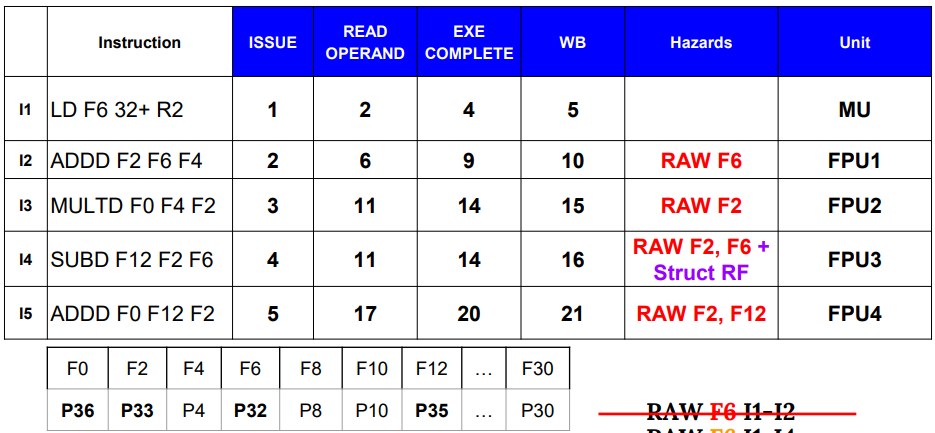
\includegraphics[width=1\linewidth]{images/tom3.png}
        \end{figure}
        The issue order is incorrect, rendering the scoreboard configuration inaccurate.
    \item Correct Scoreboard:
        \begin{figure}[H]
            \centering
            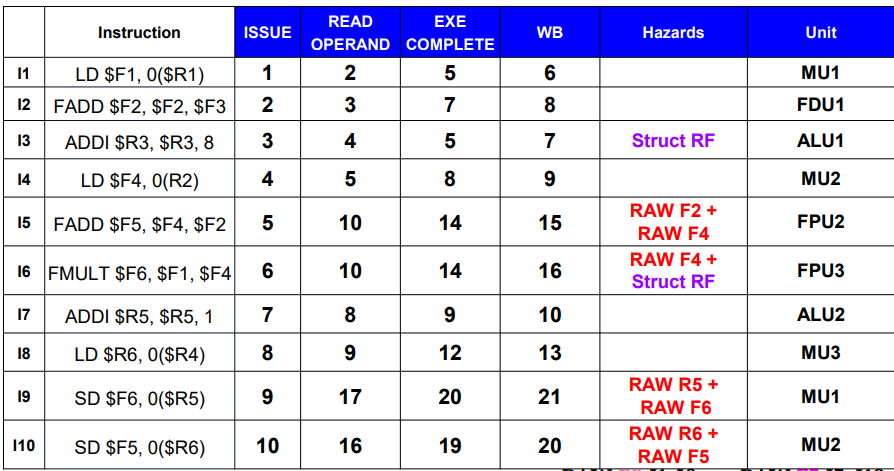
\includegraphics[width=1\linewidth]{images/score3.png}
        \end{figure}
\end{enumerate}